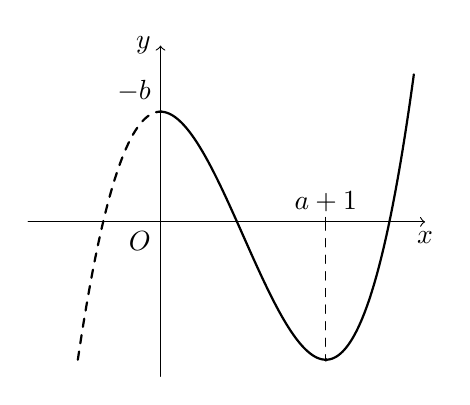
\begin{tikzpicture}[line cap=round,line join=round,scale=0.7]
\usetikzlibrary{calc,decorations.pathreplacing}

% 取参数（只用于定位；标签仍显示 -b、a+1）
\def\a{2.0}     % a>1
\def\b{-1.0}    % b<0

% 三次函数：g(x)=1/3 x^3 - 1/2(a+1)x^2 - b（把它在 x<0 处仅作“延拓示意”用虚线画）
\pgfmathsetmacro{\apone}{\a+1}
\pgfmathsetmacro{\yb}{-\b} % -b 的数值（b<0 时为正）

% 关键点：x=0 为极大点，x=a+1 为极小点
\pgfmathsetmacro{\ymax}{(1/3)*0^3 - (1/2)*(\apone)*0^2 - \b} % = -b
\pgfmathsetmacro{\ymin}{(1/3)*(\apone)^3 - (1/2)*(\apone)*(\apone)^2 - \b} % = -(a+1)^3/6 - b

% 坐标轴
\draw[->] (-2.4,0) -- (4.8,0) node[below] {$x$};
\draw[->] (0,-2.8) -- (0,3.2) node[left] {$y$};
\node[below left] at (0,0) {$O$};

% y 轴注记 -b（在 (0,-b) 处打刻度）
\draw (-0.08,\yb+1) -- (0.08,\yb+1);
\node[above left] at (0,\yb +1) {$-b$};

% x 轴注记 a+1（在 x=a+1 处打刻度）
\draw (\apone,-0.08) -- (\apone,0.08);
\node[above] at (\apone,0) {$a+1$};

% 画同一条三次曲线：x<0 虚线，x>=0 实线
\draw[dashed,thick,smooth,samples=180,domain=-1.5:0]
  plot (\x,{(1/3)*(\x)^3 - (1/2)*(\apone)*(\x)^2 - \b +1});
\draw[thick,smooth,samples=260,domain=0:4.6]
  plot (\x,{(1/3)*(\x)^3 - (1/2)*(\apone)*(\x)^2 - \b +1});

% 标出极小点处的虚线竖线（题图里那条）
\draw[dashed] (\apone,0) -- (\apone,\ymin+1);

% 点（可选：更像原图）
\fill (0,\ymax+1) circle (1.0pt);
\fill (\apone,\ymin+1) circle (1.0pt);

\end{tikzpicture}